\documentclass[aps,twocolumn,secnumarabic,balancelastpage,amsmath,amssymb]{revtex4}
\usepackage{amsmath}
\usepackage{amssymb}
\usepackage{amsfonts}
\usepackage{color}
\usepackage{graphics}
\usepackage[pdftex]{graphicx}
\usepackage[utf8x]{inputenc}
\usepackage[colorlinks=true]{hyperref}

\newcommand{\ud}{\mathrm{d}}
\newcommand{\ue}{\mathrm{e}}
\newcommand{\ui}{\mathrm{i}}
\newcommand{\res}{\mathrm{Res}}
\newcommand{\Tr}{\mathrm{Tr}}
\newcommand{\dsum}{\displaystyle\sum}
\newcommand{\dprod}{\displaystyle\prod}
\newcommand{\dlim}{\dispqlaystyle\lim}
\newcommand{\dint}{\displaystyle\int}
\newcommand{\fsno}[1]{{\!\not\!{#1}}}
\newcommand{\texp}[2]{\ensuremath{{#1}\times10^{#2}}}
\newcommand{\dexp}[2]{\ensuremath{{#1}\cdot10^{#2}}}
\newcommand{\eval}[2]{{\left.{#1}\right|_{#2}}}
\newcommand{\paren}[1]{{\left({#1}\right)}}
\newcommand{\lparen}[1]{{\left({#1}\right.}}
\newcommand{\rparen}[1]{{\left.{#1}\right)}}
\newcommand{\abs}[1]{{\left|{#1}\right|}}
\newcommand{\sqr}[1]{{\left[{#1}\right]}}
\newcommand{\crly}[1]{{\left\{{#1}\right\}}}
\newcommand{\angl}[1]{{\left\langle{#1}\right\rangle}}
\newcommand{\tpdiff}[4][{}]{{\paren{\frac{\partial^{#1} {#2}}{\partial {#3}{}^{#1}}}_{#4}}}
\newcommand{\tpsdiff}[4][{}]{{\paren{\frac{\partial^{#1}}{\partial {#3}{}^{#1}}{#2}}_{#4}}}
\newcommand{\pdiff}[3][{}]{{\frac{\partial^{#1} {#2}}{\partial {#3}{}^{#1}}}}
\newcommand{\diff}[3][{}]{{\frac{\ud^{#1} {#2}}{\ud {#3}{}^{#1}}}}
\newcommand{\psdiff}[3][{}]{{\frac{\partial^{#1}}{\partial {#3}{}^{#1}} {#2}}}
\newcommand{\sdiff}[3][{}]{{\frac{\ud^{#1}}{\ud {#3}{}^{#1}} {#2}}}
\newcommand{\tpddiff}[4][{}]{{\left(\dfrac{\partial^{#1} {#2}}{\partial {#3}{}^{#1}}\right)_{#4}}}
\newcommand{\tpsddiff}[4][{}]{{\paren{\dfrac{\partial^{#1}}{\partial {#3}{}^{#1}}{#2}}_{#4}}}
\newcommand{\pddiff}[3][{}]{{\dfrac{\partial^{#1} {#2}}{\partial {#3}{}^{#1}}}}
\newcommand{\ddiff}[3][{}]{{\dfrac{\ud^{#1} {#2}}{\ud {#3}{}^{#1}}}}
\newcommand{\psddiff}[3][{}]{{\frac{\partial^{#1}}{\partial{}^{#1} {#3}} {#2}}}
\newcommand{\sddiff}[3][{}]{{\frac{\ud^{#1}}{\ud {#3}{}^{#1}} {#2}}}
\newcommand{\eff}{ef\! f}

\begin{document}
\title{Motional Quantum Ground-State Cooling Outside the Lamb-Dicke Regime -- Supplemental material}
\author{Yichao Yu}
\author{Nicholas R. Hutzler}
\author{Jessie T. Zhang}
\author{Lee R. Liu}
\author{Kang-Kuen Ni}
\email{ni@chemistry.harvard.edu}
\affiliation{Department of Chemistry and Chemical Biology, Harvard University, Cambridge, Massachusetts, 02138, USA}
\affiliation{Department of Physics, Harvard University, Cambridge, Massachusetts, 02138, USA}
\affiliation{Harvard-MIT Center for Ultracold Atoms, Cambridge, Massachusetts, 02138, USA}

\date{\today}

\maketitle

\section{Simulation of 3D Raman sideband cooling}

\subsection{Overview}

We use a computer simulation to study the importance of different effects
and guide the optimization of cooling.
The simulation uses quantum jump method\cite{Chretien2014} (or Monte-Carlo wavefunction method)
to accurately calculate the evolution within each laser pulse while different energy eigenstates
are assumed to decohere immediately on spontaneous emission of photon and on pulse boundaries.
Such approxiations are valid for simulation of the cooling and greatly simplifies the computation
at the cost of limiting the applicability of the simulation to processes that requires stronger
coherence such as Ramsey spectroscopy and rapid push-out.

A few other approximations are used in the simulation either because they are proved to have
negligible effect on the experiment or because they'll increase the complexity of the simulation
and can be optimized through other methods in the experiment.
A list of the most important approximations is,

\begin{enumerate}
\item All Raman pulses are assumed to be resonantly driving only one sideband/carrier order.\\
  We tweak the pulse shape, power and length to suppress any deviation
  from this in the experiment. We do still see deviation from this in the experiment
  but the effect is small for the short pulse we use for cooling and is the most pronounced
  for long detection pulses.
\item No heating from other sources including trap switching.\\
  We measured the heating rate and observed that it mainly comes from off-resonance scattering
  of photons from various sources which we already include so additional heating can be
  ignored.
\item Trapping frequency difference between different states are ignored.\\
  This effect is negligible for Na in the ground state due to the small fine structure.
  It is easy to include this effect if the calculation needs to be repeated on a system where
  this is not the case (e.g. directly laser cooled molecules)
\end{enumerate}

Some of the important effects that are included are,
\begin{enumerate}
\item Full 3D simulation.\\
  This includes 3D motional states, accurate 3D wavevector, and different emission pattern
  for different photon polarizations.
\item Off resonant scattering from all beams.\\
  Including Raman, optical pumping and dipole trap.
\item Optical pumping polarization imperfection.
\end{enumerate}

The optical pumping polarization and the off resonant scattering are especially important
for accurate simulation since they are the main heating source that is present
for ground motional dark state atom and therefore are the main limation on cooling performance.

\subsection{Simulation of each pulse}

Each pulse in general has a coherent part from the Raman drive (zero for optical pumping pulse)
and an incoherent part from scattering (optical pumping or off-resonance scattering).
This nicely fits the general formula of the quantum jump method. Due to the large number of
states that we need to take into account ($30-150$ states in each of the three axis and
$8$ hyperfine states, giving a total of $10^6$ states),
the generic wavefunction propagation is very inefficient.
Therefore, this is further simplified by reducing the number of states to be kept track of during
the coherent propagation and apply quantum jump using a set of reduced jump operator that
describes the total jump probability from a certain states (sum over all final states).
The coherent propagation is then accurately solved in order to avoid having to use a time step
much shorter than the scattering rate (up to hundreds of kHz)\footnote{\href{https://goo.gl/EZ13wt}{note about modification to the quantum jump method (https://goo.gl/EZ13wt)}}.

In order to simulate a pulse, we first start with the coherent propagation that includes the
modification from the jump operators as in quantum jump method.
When a jump happens, we pick a final internal state to jump to based on the rates ratio
of different scattering sources and their branching ratios.
This process also determines the polarization and emission pattern of the photon and
a particular wave vector for the emitted photon is then selected as the next step.
The recoil is not fixed so the final motional state of the atom can now be selected.
This process is then repeated on the same pulse until the pulse time is used up before
we start to simulate the next pulse.

\subsection{Measurements}

We apply ``virtual'' measurements on each results of the cooling which we then average to
obtain the expected value of qualities that we are interested in.
Due to the decoherence approximation, the measurement has to commute with the Hamiltonian.
Particularly useful measurements used in our simulation are hyperfine state distribution,
Average motional energy, loss rate (where an atom is assumed to be lost if its motional energy
goes above a certain threshold at any time) probability of being in certain states
(e.g. ground state).

\subsection{Sample results}

\begin{figure}
  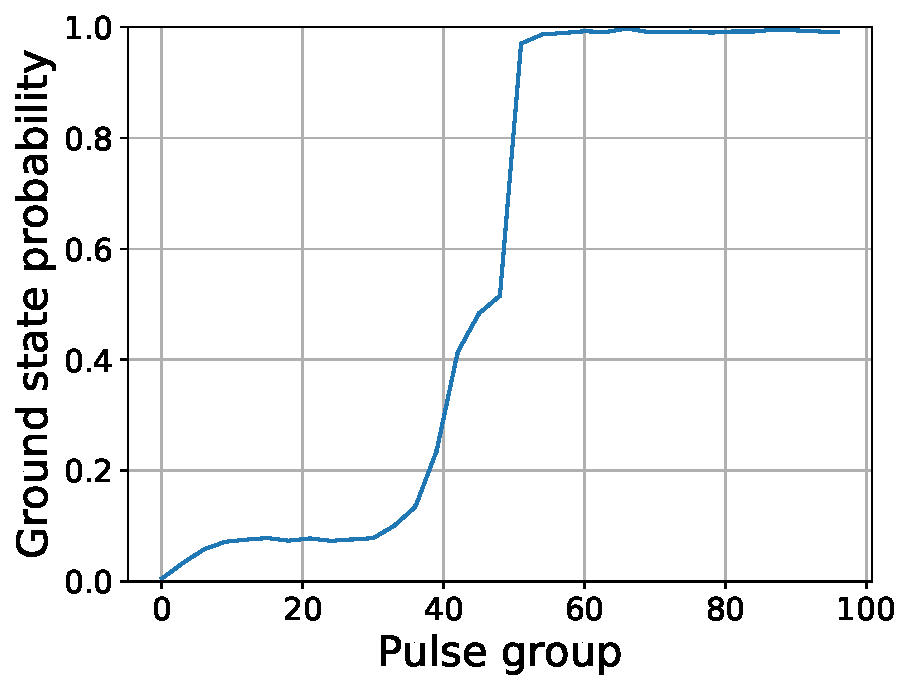
\includegraphics[width=8.5cm]{imgs/simcool_no_scatter.pdf}
  \caption{Simulated ground state population as a function of cooling cycles without
    technical imperfections. The ground state probability reaches $>99\%$. \label{f-no-scatter}}
\end{figure}

\begin{figure}
  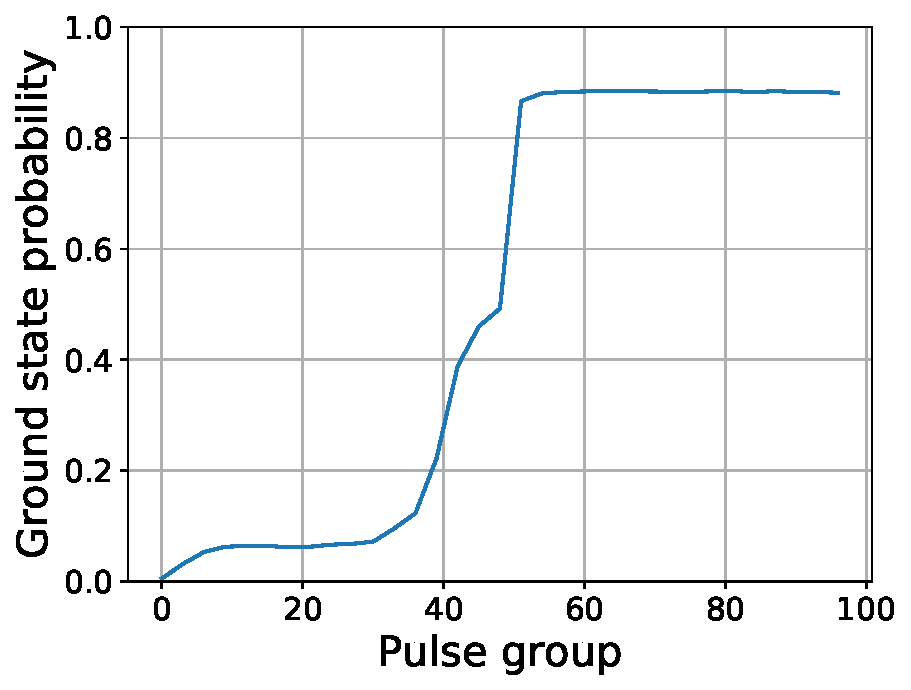
\includegraphics[width=8.5cm]{imgs/simcool_real.pdf}
  \caption{Simulated ground state population as a function of cooling cycles including effect of
    off-resonant scattering from all beams and OP misalignment.
    For this particular sequence, the ground state probability saturates $\approx88\%$.
    \label{f-real}}
\end{figure}

When not considering the off-resonant scattering from the Raman beams and the tweezer as well
as optical pumping polarization misalignment, the simulation shows that there isn't a cooling
limit despite the large Lamb-Dicke parameter and high initial temperature (Fig \ref{f-no-scatter}).
However, when these effects are taken into account, the ground state probability can saturate at
a lower value (Fig \ref{f-real}) and require much more careful tweaking.

\subsection{Code}

The simulation is written in Julia. All code are available under GPLv3 license at
\footnote{\href{https://goo.gl/WLJwJp}{Library code (https://goo.gl/WLJwJp)}} and
\footnote{\href{https://goo.gl/XXVreq}{Top level code (https://goo.gl/XXVreq)}}

\bibliography{paper}
\end{document}
